\documentclass{article}\usepackage[]{graphicx}\usepackage[]{color}

\usepackage{alltt}
\usepackage{float}
\usepackage{graphicx}
\usepackage{tabularx}
\usepackage{siunitx}
\usepackage{amssymb} % for math symbols
\usepackage{amsmath} % for aligning equations
\usepackage{textcomp}
\usepackage{booktabs}
\usepackage{mdframed}
\usepackage{natbib}
\usepackage{comment}
\usepackage[colorinlistoftodos]{todonotes} % to make comments on the margin
\usepackage[small]{caption}
\setlength{\captionmargin}{30pt}
\setlength{\abovecaptionskip}{0pt}
\setlength{\belowcaptionskip}{10pt}
\topmargin -1.5cm        
\oddsidemargin -0.04cm   
\evensidemargin -0.04cm
\textwidth 16.59cm
\textheight 21.94cm 
%\pagestyle{empty} %comment if want page numbers
\parskip 7.2pt
\renewcommand{\baselinestretch}{1.5}
\parindent 0pt
%\usepackage{lineno}
%\linenumbers

%% R Script

\title{Evolution constrains tree responses to environmental cues in experimental settings too - Outline\\
			or\\
			Revisiting the Phylogenetic Mixed Model}

\begin{document}

\maketitle

\noindent Authors:\\
The Wolkovich Lab in 2019 $^{1,2,3,4}$
\vspace{2ex}\\
\emph{Author affiliations:}\\
$^{1}$Forest \& Conservation Sciences, Faculty of Forestry, University of British Columbia, 2424 Main Mall, Vancouver, BC V6T 1Z4;\\
$^{2}$Arnold Arboretum of Harvard University, 1300 Centre Street, Boston, Massachusetts, USA;\\
$^{3}$Organismic \& Evolutionary Biology, Harvard University, 26 Oxford Street, Cambridge, Massachusetts, USA;\\
$^{4}$Edificio Ciencias, Campus Universitario 28805 Alcalá de Henares, Madrid, Spain\\
 

\vspace{2ex}
$^*$Corresponding author: ignacio.moralesc@uah.es\\
\renewcommand{\thetable}{\arabic{table}}
\renewcommand{\thefigure}{\arabic{figure}}
\renewcommand{\labelitemi}{$-$}
\setkeys{Gin}{width=0.8\textwidth}

%%%%%%%%%%%%%%%%%%%%%%%%%%%%%%%%%%%%%%%%%%%%%%%
%%%%%%%%%%%%%%%%%%%%%%%%%%%%%%%%%%%%%%%%%%%%%%%
\clearpage
\section*{Rationale \& Significance}

Previous work has looked at the phylogenetic conservatism of phenology across plant species, finding that, first flowering is significantly conserved \citep{davies2013phylogenetic} and, when using OU models so are shifts in first flowering and the slopes of the relationship between flowering and year \citep{rafferty2017global}. Research in this area has focused on the phenotype (phenological event or its shifts) rather than on the cues---i.e. how shifts in the environment trigger species responses. Beyond whether or not phenology is phylogenetically conserved, determining evolutionary constraints in phenological responses to temperature and daylight, may have deeper implications for forecasting under ongoing change.\\ 

Nevertheless, previous work on the phylogenetic conservatism of phenology has still not addressed:\\

- Emphasis has been put on the phenotype rather than on the cues\\
- Are phenological responses in lab experiments conserved as well? In \cite{joly2019importance} the authors check this with a focus on intraspecific variations\\
- How the sensitivities to different environmental cues are conserved?\\
- Are the responses to certain cues more strongly conserved than to others?\\
- How does accounting for phylogeny affects model estimations of cue sensitivity?\\

And beyond work on phylogenetic conservatism, previous comparative research on phenological responses to cues (experimental or observational) has either:\\

- Ignored phylogenetic relationships (or the fact that species are not independent units)\\
- Accounted for phylogenetic relationships assuming that they are \emph{stationary} across predictors-traits and can be modelled by including phylogenetic Variance-Covariance in model residuals. This is the rationale behind common-use PGLS approaches but it \"hides\" the partial phylogenetic constraints to model predictors.\\ 

An overlooked question so far is whether we could gain any additional information by accounting for independent phylogenetic structuring in each species responses to each predictor in a multi-linear response model setting. Typical methods are good to account for species non-independence but provide little insight relative to phylogenetic effects on each predictor.
\todo{I think the new approach is a bit of a game changer as it shifts the focus from empirical results of phylo-constrains on phenology to a more methodsy paper. We need to decide a focus.}



The potential interest of findings in this direction stem from:\\
- better predictions of phenology (or need to account for it in models)\\
- better understanding of the mechanistic basis of plant responses to climate\\
- better design the next generation of experiments \\



%%% A few notes/questions from close reading of Housworth et al. 2004
% - should we change the terminology (lambda) to that in Housworth? H²?
% - should we care about rho correlations between traits (cues)? if so, they can be estimated through sigma2 and h2 given that h2 = sigma2_inherited / sigma2. 
% 


\section*{Abstract}
\begin{enumerate}

Plants have long evolved responses to environmental cues, able to inform the organisms about the temporal distribution of key resources---i.e. energy and light. The plasticity of these responses may ultimately determine species ability to withstand ongoing environmental change because non-plastic species may undergo developmental events under unadequate conditions---e.g. a species advancing flowering too much could see increased the risk of frost events. Phenology describes the responses to seasonal change in environmental cues and while it is often regarded to as a rather plastic trait, it is still unknown whether or not phenology is a phylogenetically conserved trait. Here we use Bayesian hierarchical models and the most complete dataset on tree species phenological responses measured in experimental conditions to: (a) test if tree species responses to cues are conserved phylogenetically, (b) compare the phylogenetic signal in the responses to different cues and, (c) test the abiltiy of phylogenetically informed models to improve predictive accuracy of phenology. Results show non-random phylogenetic structuring of phenological responses, highly variable across cues.  
Taken together, our results suggest that phylogeny should be incorporated into studies modelling multi-species phenological responses, as such responses have been constrained through evolution and thus are not independent.  

\item How plants respond to environmental cues--i.e. temperature, daylight--may determine their resilience or vulnerability to ongoing climate change. 
\item Phenology provides a good description of plant responses to to the environment. 
\item Phenology has been regarded to as a rather plastic trait, thus with a lot of variation both intra- and inter-specifically.
\item Variation in phenology could have randomly accummulated across species (and then phenology would be an evolutionary labile trait), or be structured in the phylogeny so that closely related species resemble more each other in their phenological responses (conserved trait).
\item Whether or not phenology is conserved has implications for the need to account for phylogenetic autocorrelation in cross-species analyses.
\item More interestingly, given that phylogeny can act as a proxy for other (unaccounted) traits that may be linked to phenology, including it in models could lead to more accurate predictions.
\item Here we use Bayesian hierarchical models and the most complete dataset on tree species phenological responses measured in experimental conditions to: (a) test if tree species responses to cues are conserved phylogenetically, (b) compare the phylogenetic signal in the responses to different cues and, (c) test the abiltiy of phylogenetically informed models to improve predictive accuracy of phenology.
\item Results show non-random phylogenetic structuring of phenological responses, highly variable across cues.  
\item Taken together, our results suggest that phylogeny should be incorporated into studies modelling multi-species phenological responses, as such responses have been constrained through evolution and thus are not independent.  
\end{enumerate}

% not yet satisfied about the pitch - this is already said in Davies et al. 2013 
% should we emphasize the fact that we are using experimental/lab data? What are the gains with respect data from the field?

% we need an angle of at least some novelty

%%%%%%%%%%%%%%%%%%%%%%%%%%%%%%%
% Introduction
%%%%%%%%%%%%%%%%%%%%%%%%%%%%%%%

\section*{Introduction}
\begin{enumerate}
\item Phenology is a critical trait to studying biological responses to climate change.
\item Forecasts of phenological responses to environmental change are very important (e.g. agriculture, pest management, etc.) but they are not successful, partly due to data limitations: many species lack data and even those with data may have incomplete time series for all relevant phenophases. Could we impute missing data using phylogeny as a proxy? Even if we have the data, should multi-species forecasts be concerned with phylogenetic constraints? 
\item Phenology has been shown to be phylogenetically conserved, but studies to date are limited by:
\begin{enumerate}
\item focused on flowering (and leafout some) times and shifts in them (but see \cite{joly2019importance}, and add REFs!! on other phenological stages: budburst, ripening)
\item studied trait correlation \citep{bolmgren2008time} (not a limitation, but a different focus)
\item studied different evolutionary models best fitting the data \citep{rafferty2017global}
\item measured shifts based on field observation data for both climate and phenology (when slopes are available, they represent shifts with time, not shifts with the environment).
\item most efforts are on the phenotype rather than on the magnitude of species phenological responsiveness to different environmental cues.
\end{enumerate}
\item Few examples in the literature have tested for phylogenetic signal of phenological responses using growth chamber data (e.g. \cite{joly2019importance}, and yet such a source of data could have advantages such as:
\begin{enumerate}
\item it makes possible to examine responses to more than one cue and thus not restrict analyses to responses to forcing.
\item it is possible to compare responses to cues (are some more conserved than others?) 
\item they may allow testing whether phylogeny can improve models of phenology as a response to a cue
\end{enumerate}

\item Shifting the focus to phylogenetic conservatism of the responses to cues may provide additional insights:
\begin{enumerate}
\item by allowing comparison across cues, which cues are more conserved? which selective processes have been stronger? 
\item Do we need to care about phylogenetic constraints when we forecast phenology? 
\item Understand what dimensions of the environment may be more limiting or may be less subject to further adaptation. 
\item Is the phylogenetic conservatism of phenology affected by geography and/or taxonomy? (e.g. North America vs. Europe; Gymnosperms vs. Angiosperms) 
\end{enumerate}

\item Here we use the largest dataset on experimental phenology to model species responses to three major environmental cues---i.e. forcing, chilling, photoperiod---and test their. We expect non-random phylogenetic conservatism of the cues based on previous research \citep{davies2013phylogenetic,rafferty2017global,joly2019importance} and expect that temperature-related cues display higher phylogenetic signal than photoperiod because the latter has remained more constant through evoutionary time. % it still needs hypotheses/predictions about the forecasts TBD

\end{enumerate}
\todo{The intro topics need punch and relevant antecedents (I'm still getting acquainted with the literature), help with bibliographic review of the topic would be awesome}



\clearpage


%%%%%%%%%%%%%%%%%%%%%%%%%%%%%%%
% Methods
%%%%%%%%%%%%%%%%%%%%%%%%%%%%%%%

\section*{Methods}
\subsection*{Phenological and Phylogenetic Data}
\begin{enumerate}
\item Description of the OSPREE database (where it comes from, number of species, studies, etc.).  
\todo{Help here would be much appreciated!}

\item We analyze 5 different subsets of species in the OSPREE database to explore differences across taxa (effect of gymnosperms?) and to test to what extent data resolution affects the results:

\begin{enumerate}
\item Species grouped in generic complexes, to ensure enough cross-treatment data, as in Ettinger et al. (under review) (including 52 complexes)[flags.for.mainmodel=T]
\item All species in the main model (including 117 species resulting from )[flags.for.mainmodel=T]
\item All angiosperm species in the main model (including 110 species)[flags.for.mainmodel=T]
\item All species in the latest version of OSPREE (including 231 species resulting from )[flags.for.allsppmodel=T]
\item All angiosperm species in the latest version of OSPREE (including 215 species)[flags.for.allsppmodel=T]
\end{enumerate}

\item Two phylogenetic hypotheses have been considered to build a tree containing the species in OSPREE. First the vascular plant megatree by Zanne et al. (2014);Nature and, second the megatree by Smith \& Brown (2019);AJB. 

\item The backbone phylogenies were pruned to contain only the studied species in each subset.  

\item Species not in the backbone phylogeny were added as polytomies at the generic level ( using the function \emph{congeneric.merge}; \citep{pearse2015pez}).  

\item To build a phylogeny for species complexes, the terminal branches of species belonging to the same complexes were collapsed.  

\end{enumerate}

\subsection*{Provenance-climate Data}
\begin{enumerate}
\item Should we test/analyze provenace or climate-effects? 
\todo{I belive this can be done (roughly) through the NAm vs. Eur comparison?} 
\end{enumerate}




\subsection*{The Bayesian hierarchical phylogenetic model}

%The following text is literally copied from Geoff's

For each of $n$ species, we assumed that data were generated from the following sampling distribution:

\begin{align}
  \label{modely}
  y_j \sim \mathcal{N}(\mu_j, \sigma_e^2)
\end{align}
where
\begin{align}
  \label{modelmu}
  \mu_j = \alpha_j + \beta_{1,j} X_2 + \beta_{2,j} X_2 + \beta_{3,j} X_3
\end{align}

Predictors $X_1$, $X_2$, $X_3$ are standardized forcing, chilling, and photoperiod, and their effects on the phenology of species $j$ are determined by parameters $\beta_{1,j}$, $\beta_{2,j}$, $\beta_{3,j}$ representing traits. These traits, including the species-specific intercept $\alpha_j$, are elements of the following normal random vectors:
\begin{align}
  \boldsymbol{\alpha} = \{\alpha_1, \ldots, \alpha_n\}^T & \text{ such that }
  \boldsymbol{\alpha} \sim \mathcal{N}(\mu_{\alpha},\boldsymbol{\Sigma_{\alpha}}) \\
  \boldsymbol{\beta_1} =  \{\beta_{1,1}, \ldots, \beta_{1,n}\}^T & \text{ such that }
  \boldsymbol{\beta_1} \sim \mathcal{N}(\mu_{\beta_1},\boldsymbol{\Sigma_{\beta_1}}) \nonumber \\
  \boldsymbol{\beta_2} =  \{\beta_{2,1}, \ldots, \beta_{2,n}\}^T & \text{ such that }
  \boldsymbol{\beta_2} \sim \mathcal{N}(\mu_{\beta_2},\boldsymbol{\Sigma_{\beta_2}}) \nonumber \\
  \boldsymbol{\beta_3} =  \{\beta_{3,1}, \ldots, \beta_{3,n}\}^T & \text{ such that }
  \boldsymbol{\beta_3} \sim \mathcal{N}(\mu_{\beta_3},\boldsymbol{\Sigma_{\beta_3}}) \nonumber
\end{align}

\noindent where the means of the multivariate normal distributions are root trait values (i.e., trait values prior to evolving across a phylogenetic tree) and $\boldsymbol{\Sigma_i}$ are $n \times n$ phylogenetic variance-covariance matrices of the form: \\

\begin{align}
  \label{phymat}
\begin{bmatrix}
  \sigma^2_i & \lambda_i \times \sigma_{i} \times \rho_{12} & \ldots & \lambda_i \times \sigma_{i} \times \rho_{1n} \\
  \lambda_i \times \sigma_i \times \rho_{21} & \sigma^2_i & \ldots & \lambda_i \times \sigma_{i} \times \rho_{2n} \\
  \vdots & \vdots & \ddots & \vdots \\
  \lambda_i \times \sigma_i \times \rho_{n1} & \lambda_i \times \sigma_i \times \rho_{n2} & \ldots & \sigma^2_i \\
\end{bmatrix}
\end{align}

\noindent where $\sigma_i^2$ is the rate of evolution across a tree for trait $i$ (here assumed to be constant along all branches), $\lambda_i$ scales branch lengths and therefore is a measure of the ``phylogenetic signal'' within a species trait, and $\rho_{xy}$ is the phylogenetic correlation between species $x$ and $y$, or the fraction of the tree shared by the two species.

The above specification is exactly equivalent to writing equation \ref{modelmu} in terms of root trait values and residuals, such that:

\begin{align}
  \mu_j = \mu_\alpha + \mu_{\beta_1} X_1 + \mu_{\beta_2} X_2 + \mu_{\beta_3} X_3 + e_{\alpha_{j}} + e_{\beta_{1,j}} + e_{\beta_{2,j}} + e_{\beta_{3,j}}
\end{align}

\noindent where the residual error terms (e.g., $e_{\alpha_{j}}$) are elements of normal random vectors from multivariate normal distributions centered on $0$ with the same phylogenetic variance-covariance matrices as in equation \ref{phymat}.


\subsection*{Interpretation of \lambda_i}

\item In contrast to classic approaches to controlling for phylogenetic non-independence of analysis units (i.e. species), see \citep{freckleton2002phylogenetic}, where Pagel's \cite{pagel1999inferring} $\lambda$ is assumed constant across multiple predictors if those enter a PGLS model, our approach retrieves 

\item The $\lambda$ in our models is analogous to, but not fully equivalent to Pagel's \cite{pagel1999inferring} $\lambda$ parameter \citep{housworth2004phylogenetic}, constrained to range from 0 to 1, with values of 0 indicating absence of phylogenetic relatedness, and values of 1 indicating \emph{Brownian Motion} evolution (BM). This is because in our approach, a $\lambda$  is estimated for each predictor in the model whilst in PGLS and similar approaches, $\lambda$ is computed simultaneously across the predictor matrix. 


% for $\lambda = 0$ phylogenetically close species are not more similar than phylogenetically distant species and, for $\lambda = 1$, phylogenetically close species resemble each other according to a BM model, where phenotypic variance accummulates proportional to time.
\todo{Should we compare Results from our approach and those from PGLS? - to discuss} 

%\item In other words, the $\lambda$ parameter can be defined as a scalar that multiplies the diagonal of the phylogenetic Variance-Covariance metric and that is estimated through \emph{Maximum Likelihood} in traditional comparative approaches \citep{freckleton2002phylogenetic}. Our approach, in contrast computes the ratio between amount of variance attributable to the phylogeny ($\varepsilon_{phylo}$) and the total amount of variance \ref{eq:8}.
%\todo{Results from our approach and PGLS differ in the 215spp dataset - to discuss} 

%\item We compare the results from our $H^{2}$ metric against the results for $\lambda$ computed through Phylogenetic Generalized Least Squares \citep{freckleton2002phylogenetic}. 
%\item An advantage of estimating phylogenetic signal through a Bayesian approach such as ours is that it yields a posterior distribution of $H^{2}$.




\subsection*{Phylogeny in forecasts of phenology}
This sections needs to be fleshed out, but first we need to think and decide how to proceed (or if we want to proceed at all):

\begin{enumerate}

\item How we define the two scenarios (regular scenario; climate change scenario; see below)?
\item For which subset of species do we test it?
\item Are we predicting with and without phylogeny? I'm still not sure about how to do this.

\end{enumerate}



%%%%%%%%%%%%%%%%%%%%%%%%%%%%%%%
% Results
%%%%%%%%%%%%%%%%%%%%%%%%%%%%%%%

\section*{Results}

%\subsection*{Cue sensitivities: model accuracy and correlations across cues}
%\begin{enumerate}
%\item the model we used in the main model is the most accurate 
%\item Accuracy does not depend on whether partial pooling is on the phylogeny or on species
%\item point towards the R2 and LOO tables
%\item explain correlations across cues
%\end{enumerate}

\subsection*{Cue sensitivities: are there major shifts when phylogeny is accounted for?}

\item Perhaps we can compare the new results against those in Ailene's paper more closely \ref{fig:muplot_angio}, and \ref{fig:muplot_gymno}.

\item A first glance comparing results here with those in the NCC paper suggest that after taking phylogeny into account, the associations with photoperiod may decrease and the variance around estimations of sensitivity to chilling gets larger.



\subsection*{Phylogenetic signal in phenological responses}
\begin{enumerate}
\item Phenological responses to the three studied cues are overall phylogenetically conserved but estimates of phylogenetic signal differ strongly across species subsets (angio vs. gymno).
\item When angiosperm species (from main model) are considered, responses to forcing are more conserved ($\lambda$ = 0.64) than responses to chilling ($\lambda$ = 0.66) or to photoperiod ($\lambda$ = 0.35) (see Figure \ref{fig:phylosig_angio}).  

\item When gymnosperm species are considered, all responses to cues are similarly low (yet different from zero): forcing ($\lambda$ = 0.36), chilling ($\lambda$ = 0.32) and photoperiod ($\lambda$ = 0.37) and show almost overlapping posterior distributions, which may be driven by a low number of species (19) \ref{fig:phylosig_gymno}).  

%\item The marked differences in the responses to each cue are buffered when only angiosperm species are considered, with all responses being mildly conserved: forcing ($\lambda$ = 0.33), chilling ($\lambda$ = 0.37) and photoperiod ($\lambda$ = 0.40). This suggests gymnosperms, even few species can have a major  effect in apparent differences across cues (Figure \ref{fig:phylosig_angiosperm}). 
%\item The correlations among responses to the cues are positive but only markedly high between photoperiod and chilling (Figure \ref{fig:sensicorrs}).

\end{enumerate}


\subsection*{Budburst models, phylogenetic and non-phylogenetic}
\begin{enumerate}
\item Do we still want to do this comparison?
%\item Insert table here summarizing changes in coefficients and Rsq with/without phylogeny
\end{enumerate}



%%%%%%%%%%%%%%%%%%%%%%%%%%%%%%%
% Discussion
%%%%%%%%%%%%%%%%%%%%%%%%%%%%%%%

\section*{Discussion}
To be fleshed out.







\section*{Next steps and directions (based on Lizzie's suggestions)}
\begin{enumerate}
\item Compute phylogenetic signal on the outcome of the cues -- that is, we could calculate budburst day given our model (maybe a model without phylogeny?) under perhaps two scenarios:
     
\begin{enumerate}
\item High chill, long-ish photoperiod, and moderate forcing (regular scenario)

\item Low chill, shorter photoperiod, higher forcing (climate change scenario)

\item The trick will be first, which model to use to calculate these values and how to keep the paper then logically consistent.
\end{enumerate}
  
\end{enumerate}


\section*{Questions to be addressed}

Some questions we need to answer (suggestions by Lizzie and Nacho's addings):

\begin{enumerate}
\item How do we approach wanting to use species-level output from the models and wanting to fit phylogenetically-informed models? I think our current approach of using phylo-corrected and uncorrected models is fine, but we should discuss.
\item Do we want to compare North America and Europe somehow? sounds cool!
\item Do we want to add any traits or range stuff? - I don't think I'd go there unless there is a really pressing question or idea to address
\item Can people add refs? Especially recent refs and refs about leafout and budburst? We also should have some refs on WITHIN-species variation. This is a task that would be great if people could contribute.
\item Would it make sense to look at other response variables in OSPREE (other than budburst)?\\

And a very important question:\\

\item How do we want to pitch this paper? About phenology? About moving beyond phenotypes? About using experimental (lab) data? About climate change forecasts being affected by phylogenetic structuring?

\item If the latter, can we think of ways to show how accounting for phylogenetic structuring would affect (or best case scenario, improve) forecasts of phenology? Perhaps by focusing on well studied species (usual PEP75 suspects?)... 

\item Probably still early for this, but any ideas for target journals? JoE seems a natural outlet given where previous work has been published, but if the pitch is more into forecasts, could we aim higher?

\end{enumerate}



\bibliography{phylorefs}
\bibliographystyle{amnat}

%%%%%%%%%%%%%%%%%%%%%%%%%%%%%%%
% Tables and Figures
%%%%%%%%%%%%%%%%%%%%%%%%%%%%%%%
\section*{Tables and Figures} 


\begin{figure} [H]
  \begin{center}
  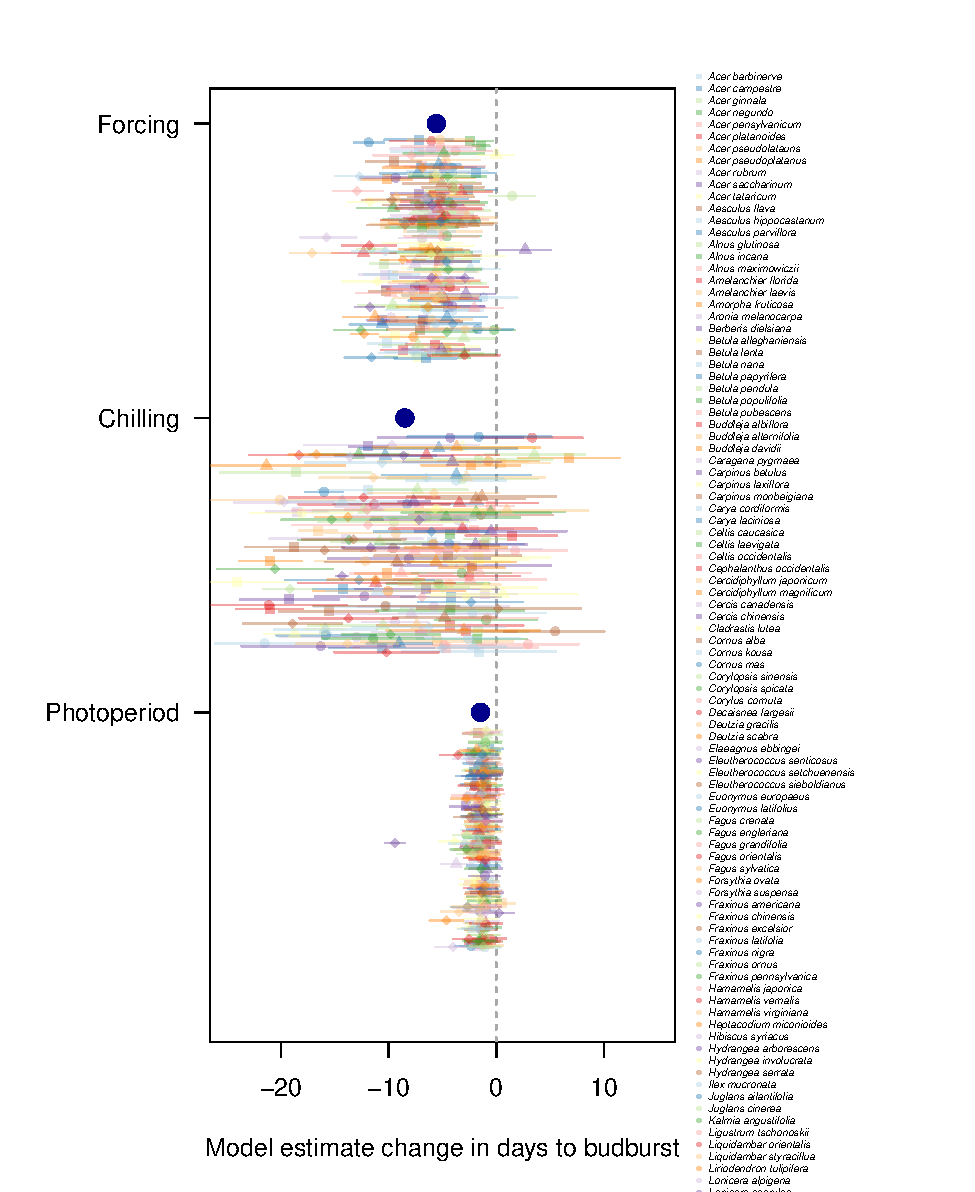
\includegraphics[width=14cm]{..//..//analyses/phylogeny/figures/muplot_angiosperm.pdf}
  \caption{Cue sensitivity estimation by hierarchical phylogenetic model showing slopes for forcing, chilling and photoperiod for 194 angiosperm species.}
  \label{fig:muplot_angio}
  \end{center}
\end{figure}

\begin{figure} [H]
  \begin{center}
  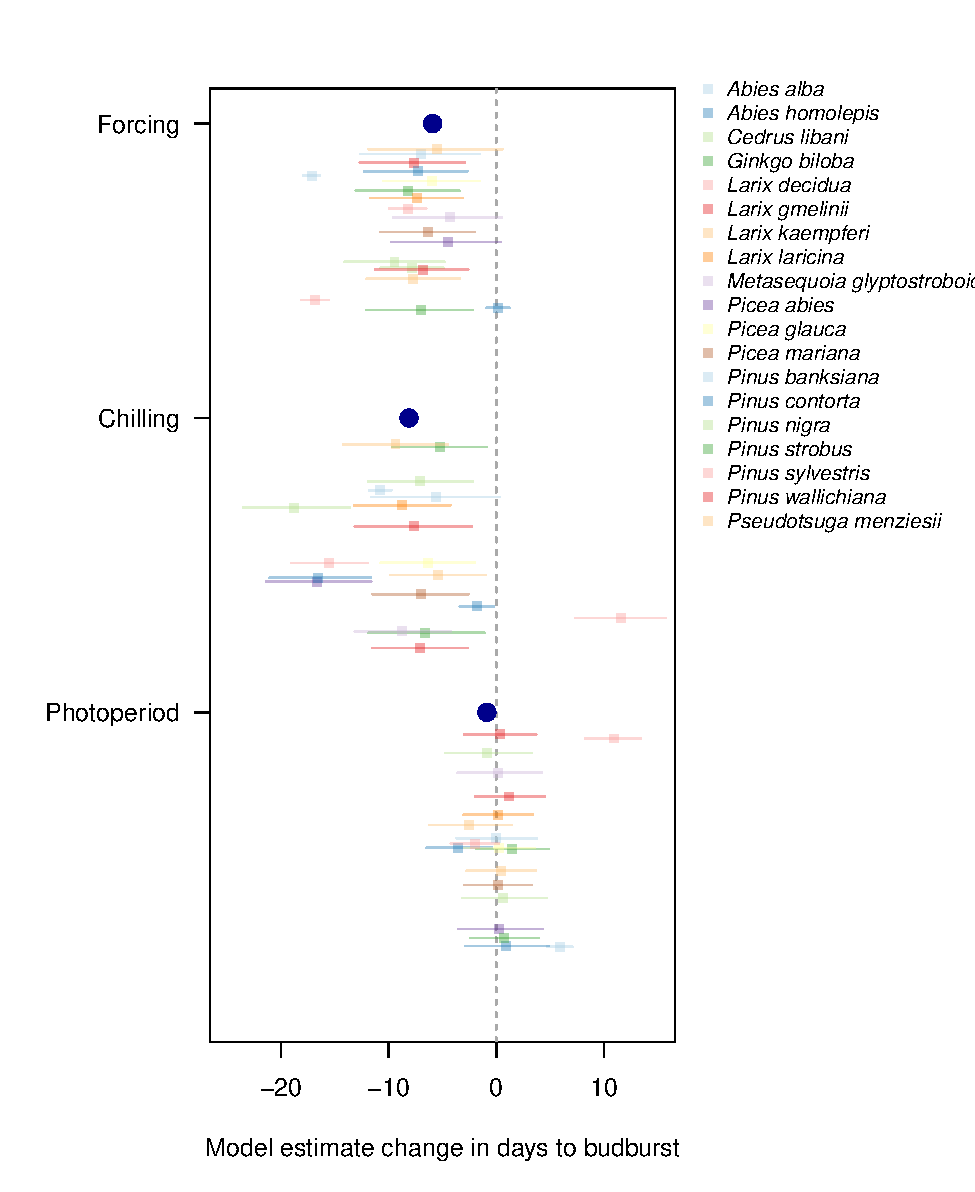
\includegraphics[width=14cm]{..//..//analyses/phylogeny/figures/muplot_gymnosperm.pdf}
  \caption{Cue sensitivity estimation by hierarchical phylogenetic model showing slopes for forcing, chilling and photoperiod for 19 gymnosperm species.}
  \label{fig:muplot_gymno}
  \end{center}
\end{figure}

\begin{figure} [H]
  \begin{center}
  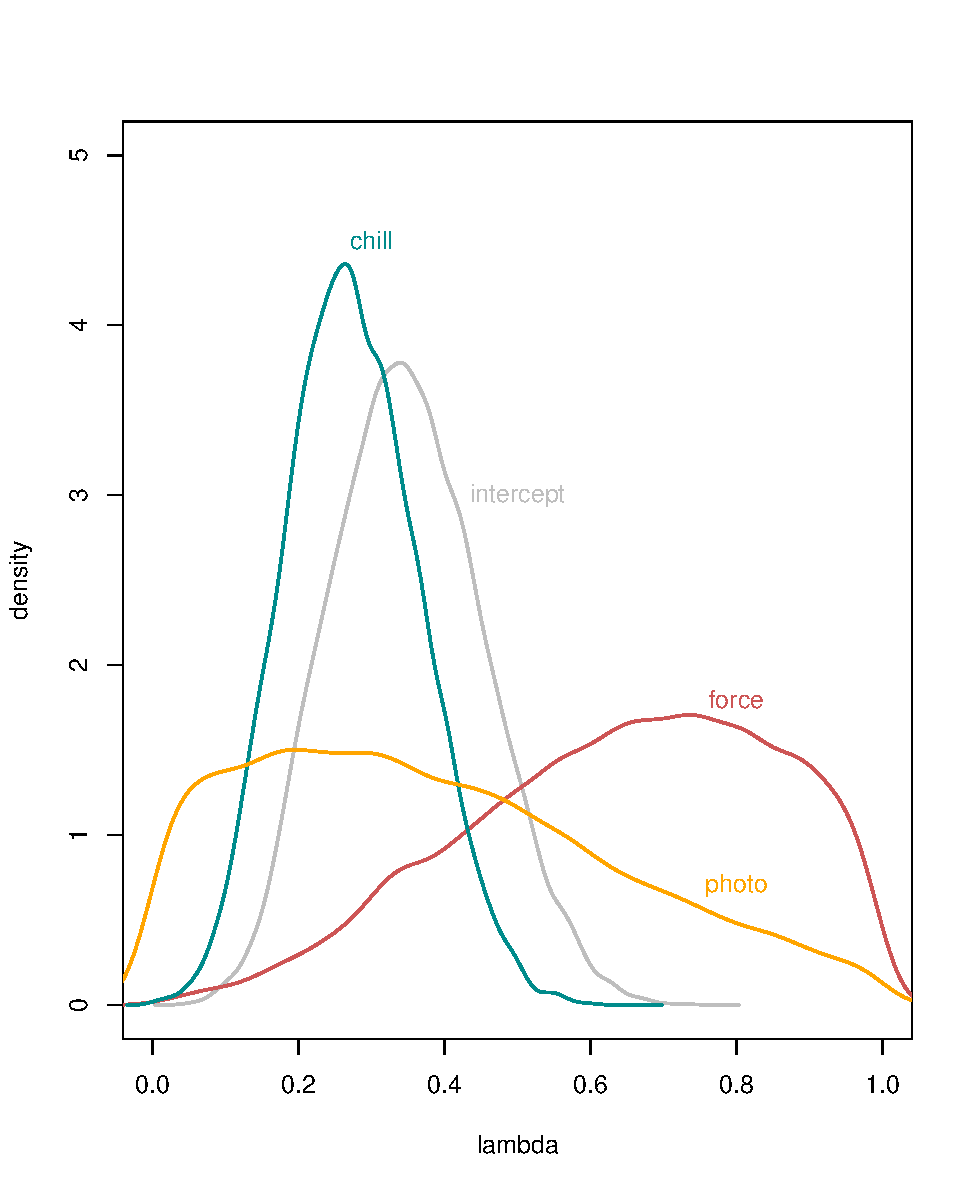
\includegraphics[width=14cm]{..//..//analyses/phylogeny/figures/lambdas_density.pdf}
  \caption{Posterior distribution of phylogenetic signal measured by lambda for each cue included as a predictor in the model for angiosperms: forcing (red), chilling (blue),  photoperiod (orange) and for the model intercept (grey).}
  \label{fig:phylosig_angio}
  \end{center}
\end{figure}

\begin{figure} [H]
  \begin{center}
  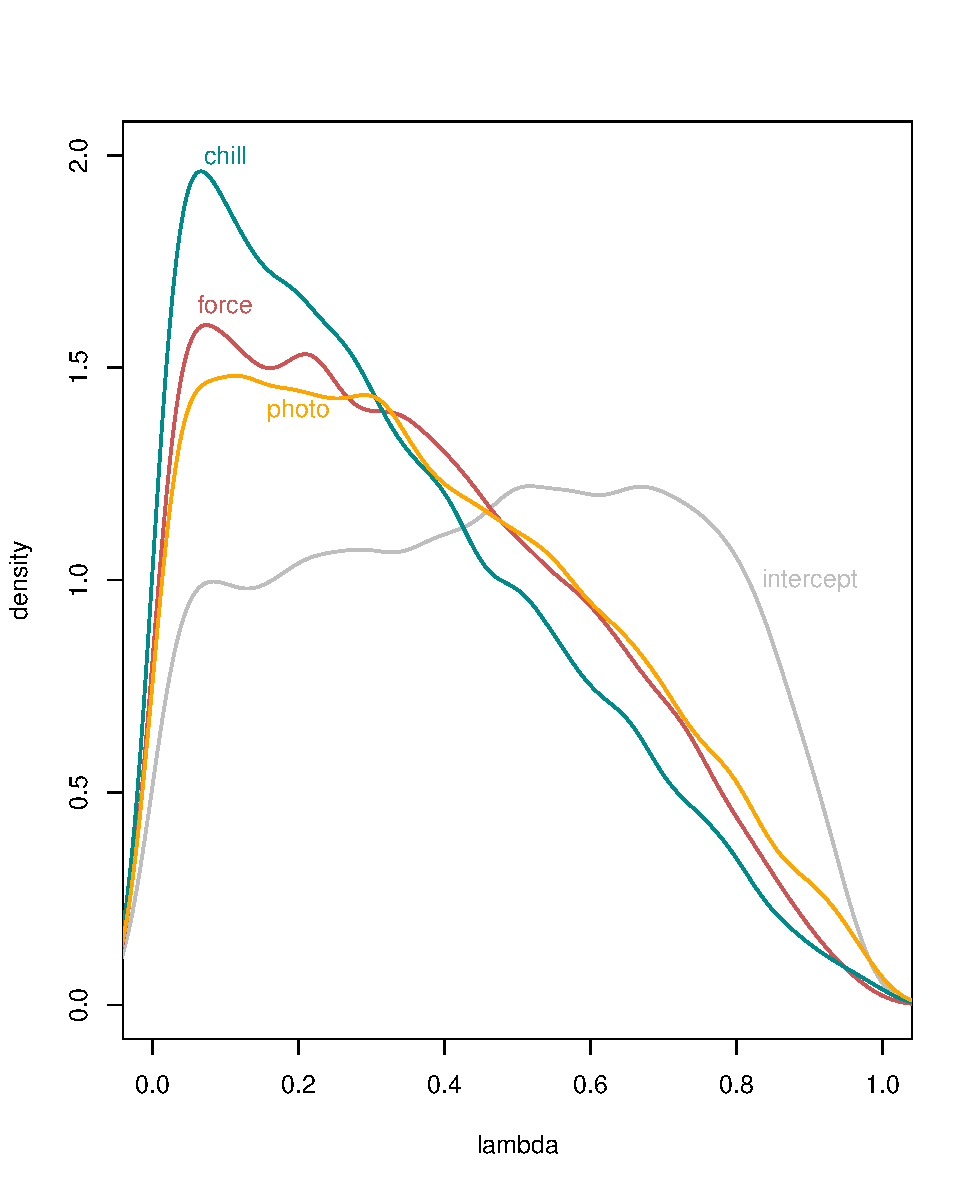
\includegraphics[width=14cm]{..//..//analyses/phylogeny/figures/lambdas_density_gymno.pdf}
  \caption{Posterior distribution of phylogenetic signal measured by lambda for each cue included as a predictor in the model for angiosperms: forcing (red), chilling (blue),  photoperiod (orange) and for the model intercept (grey).}
  \label{fig:pphylosig_gymno}
  \end{center}
\end{figure}


\begin{comment}
\begin{table}[H]
  \begin{center}

\caption{R2 estimates for models fitted to two subsets of data.}
\begin{tabular}{@{}llcccc@{}}
\toprule
Model                        & nsps & R2    & Est.Error & Q2.5  & Q97.5 \\ \midrule
mod.sps.intercept            & 52   & 0.369 & 0.012     & 0.346 & 0.392 \\
mod.sps.phylo.intercept      & 52   & 0.370 & 0.012     & 0.345 & 0.393 \\
mod.sps.interc.slope         & 52   & 0.478 & 0.011     & 0.456 & 0.498 \\
mod.sps.interc.slope.phy.int & 52   & 0.478 & 0.011     & 0.455 & 0.499 \\
mod.sps.intercept            & 117  & 0.369 & 0.012     & 0.344 & 0.393 \\
mod.sps.phylo.intercept      & 117  & 0.369 & 0.012     & 0.345 & 0.392 \\
mod.sps.interc.slope         & 117  & 0.486 & 0.011     & 0.465 & 0.506 \\
mod.sps.interc.slope.phy.int & 117  & 0.487 & 0.011     & 0.465 & 0.507 \\
mod.sps.intercept            & 215  & 0.582 & 0.007     & 0.566 & 0.596 \\
mod.sps.phylo.intercept      & 215  & 0.582 & 0.007     & 0.567 & 0.596 \\
mod.sps.interc.slope         & 215  & 0.659 & 0.006     & 0.646 & 0.670 \\
mod.sps.interc.slope.phy.int & 215  & 0.658 & 0.006     & 0.646 & 0.671 \\ \bottomrule
\end{tabular}
 \label{table:R2table}
  \end{center}

 \end{table}


\begin{table}[H]
  \begin{center}

\caption{Leave One Out analyses for models fitted to two subsets of data.}
\begin{tabular}{@{}llrrcc@{}}
\toprule
Model                        & nsps & elpd\_diff & se\_diff & elpd\_loo  & se\_elpd\_loo \\ \midrule
mod.sps.interc.slope         & 52   & 0.000      & 0.000    & -10944.890 & 75.627        \\
mod.sps.interc.slope.phy.int & 52   & -0.090     & 0.366    & -10944.980 & 75.572        \\
mod.sps.phylo.intercept      & 52   & -217.806   & 24.087   & -11162.696 & 74.662        \\
mod.sps.intercept            & 52   & -218.150   & 24.041   & -11163.040 & 74.719        \\
mod.sps.interc.slope.phy.int & 117  & 0.000      & 0.000    & -10951.579 & 75.858        \\
mod.sps.interc.slope         & 117  & -0.543     & 0.591    & -10952.122 & 75.803        \\
mod.sps.phylo.intercept      & 117  & -242.375   & 25.727   & -11193.955 & 75.031        \\
mod.sps.intercept            & 117  & -242.582   & 25.691   & -11194.161 & 75.097        \\
mod.sps.interc.slope         & 215  & 0.000      & 0.000    & -14195.898 & 89.929        \\
mod.sps.interc.slope.phy.int & 215  & -1.945     & 2.411    & -14197.843 & 90.075        \\
mod.sps.phylo.intercept      & 215  & -302.843   & 27.217   & -14498.741 & 89.759        \\
mod.sps.intercept            & 215  & -305.035   & 27.306   & -14500.933 & 89.765        \\ \bottomrule
\end{tabular}
 \label{table:lootable}
   \end{center}
\end{table}

\begin{table}[H]
\begin{center}
\caption{Comparison between phylogenetic signal from PGLS and BRMS.}
\begin{tabular}{@{}llllllll@{}}
\toprule
subset     & cue      & $\lambda$      & Lower95CI   & Upper95CI   & $H^2$          & Lower95CI   & Upper95CI   \\ \midrule
52-complex & forcing  & 0.171446841 & NA          & 0.650638627 & 0.330834872 & 0.008358609 & 0.751811447 \\
           & chilling & 1.00E-06    & NA          & 0.396954468 & 0.194753034 & 0.000682814 & 0.610910681 \\
           & photo    & 0.655354248 & 0.186405507 & 0.897899618 & 0.662218791 & 0.208150902 & 0.920502832 \\ \bottomrule
\end{tabular}
 \label{table:phylosigtable}
\end{center}
\end{table}





\clearpage
\begin{figure} [H]
  \begin{center}
  \includegraphics[width=14cm]{..//..//analyses/phylogeny/figures/correlations_sensitiv_52complex.png}
  \caption{Scatterplots showing correlations between the sensitivities of the species complexes in OSPREE to chilling and photoperiod (A), chilling and forcing (B), and forcing and photoperiod (C). Sensitivities are positively correlated among chilling and photoperiod and chilling and forcing, but negatively correlated between forcing and photoperiod.}
  \label{fig:sensicorrs}
  \end{center}
\end{figure}

\clearpage
\begin{figure} [H]
  \begin{center}
  \includegraphics[width=14cm]{..//..//analyses/phylogeny/figures/Correlations_sensitivities.png}
  \caption{Scatterplots showing correlations between the sensitivities of the species in OSPREE to chilling and photoperiod (A), chilling and forcing (B), and forcing and photoperiod (C). Sensitivities are  correlated overall, but more so between chilling and photoperiod.}
  \label{fig:sensicorrs52comp}
  \end{center}
\end{figure}

\begin{figure} [H]
  \begin{center}
  \includegraphics[width=14cm]{..//..//analyses/phylogeny/figures/cues_sensit_correlations_231spp.png}
  \caption{Scatterplots showing correlations between the sensitivities of the species in OSPREE (subset with all 231 species for which there is data) to chilling and photoperiod (A), chilling and forcing (B), and forcing and photoperiod (C). Sensitivities are positively correlated among chilling and photoperiod and chilling and forcing, but negatively correlated between forcing and photoperiod.}
  \label{fig:sensicorrs231}
  \end{center}
\end{figure}


\clearpage
\begin{figure} [H]
  \begin{center}
  \includegraphics[width=14cm]{..//..//analyses/phylogeny/figures/Sensitivities_phylosig.png}
  \caption{Phylogenetic signal results for the sensitivities of each species complex (species grouped by genera) to the forcing (A), chilling (B) and photoperiod (C) cues.}
  \label{fig:phylosig_complex}
\end{center}
\end{figure}

\begin{figure} [H]
  \begin{center}
  \includegraphics[width=14cm]{..//..//analyses/phylogeny/figures/Sensitivities_phylosig_spslev.png}
  \caption{Phylogenetic signal results for the sensitivities of each species (ungrouped) to the forcing (A), chilling (B) and photoperiod (C) cues.}
  \label{fig:phylosig_spp}
  \end{center}
  \end{figure}

\begin{figure} [H]
  \begin{center}
  \includegraphics[width=14cm]{..//..//analyses/phylogeny/figures/Sensitivities_phylosig_spslev_angiosperms.png}
  \caption{Phylogenetic signal results for the sensitivities of each species (excluding gymnosperms) to the forcing (A), chilling (B) and photoperiod (C) cues.}
  \label{fig:phylosig_angiosperm}
  \end{center}
\end{figure}

\begin{figure} [H]
  \begin{center}
  \includegraphics[width=14cm]{..//..//analyses/phylogeny/figures/Sensitivities_phylosig_spslev231.png}
  \caption{Phylogenetic signal results for the sensitivities of each species (231 species included) to the forcing (A), chilling (B) and photoperiod (C) cues.}
  \label{fig:phylosig_231spp}
  \end{center}
\end{figure}

\begin{figure} [H]
  \begin{center}
  \includegraphics[width=14cm]{..//..//analyses/phylogeny/figures/Sensitivities_phylosig_spslev215angio.png}
  \caption{Phylogenetic signal results for the sensitivities of each species (215 angiosperm only species included) to the forcing (A), chilling (B) and photoperiod (C) cues.}
  \label{fig:phylosig_215spp}
  \end{center}
\end{figure}



%%%%%%%%%%%%%%%%%%%%%%%%%%%%%%%
% Stuff from old version of the ms.
%%%%%%%%%%%%%%%%%%%%%%%%%%%%%%%
\section*{Stuff from old version (to be deleted at some point)} 

\subsection*{Hierarchical models to estimate species-level cue sensitivity}
\begin{enumerate}
\item Our approach used Bayesian hierarchical models to estimate the number of days until budburst as a function of forcing, chilling and photoperiod. We used different specifications of partial pooling to determine in which approach the sensitivies to the cues most accurately predict budburst. We used 5 model specifications: 
\begin{enumerate}
\item species as a grouping factor on the intercept (Eq. \ref{eq:1})
\item species as grouping factor on the intercept and slopes too (Eq. \ref{eq:2})
\item phylogeny as a grouping factor on the intercept and species as grouping factor on both  intercept and slopes (Eq. \ref{eq:3})
\item phylogeny as a grouping factor on the intercept and species as grouping factor on both  intercept and slopes (Eq. \ref{eq:3})

\end{enumerate}

\item In all specifications, the Bayesian hierarchical models were fit using the brms package \citep{brms}, in R \citep{R}, version 3.5.1, and followed the notations: 


\begin{equation}
\label{eq:1} 
Budbreak = \alpha_{species} + \beta_{1}forcing 
+ \beta_{2}chilling + \beta_{3}photo + \varepsilon
\end{equation}


\begin{equation} 
\label{eq:2} 
Budbreak = \alpha_{spp} + \beta_{1,spp}forcing
+ \beta_{2,spp}chilling + \beta_{3,spp}photo + \varepsilon\end{equation}

\begin{equation} 
\label{eq:3} 
Budbreak = \alpha_{phylo,spp} + \beta_{1,spp}forcing
+ \beta_{2,spp}chilling + \beta_{3,spp}photo + \varepsilon
\end{equation}

\begin{equation} 
\label{eq:4} 
Budbreak = \alpha_{phylo,species} + \beta_{1}forcing
+ \beta_{2}chilling + \beta_{3}photo + \varepsilon
\end{equation}

% I'm ignoring the model below for now as it runs very slow, and it does not seem like we are using it
%\begin{equation} 
%\label{eq:5} 
%Budbreak = \alpha_{phylo,spp} + \beta_{1, phylo, spp}forcing +\\
% \beta_{2, phylo, spp}chilling + \\
% \beta_{3, phylo, spp}photo + \varepsilon
%\end{equation}


\item We assessed model performance according to $\hat{R}$ values (that should be close to one to ensure convergence). As for metrics of model accuracy we computed $R^{2}$, and the expected log predictive density (ELPD) that results from \emph{Leave-one-out} cross-validation, in addition to inspection of posterior predictive checks.

\item To test the ability of phylogeny to improve models/predictions of budburst we compared metrics of model accuracy between models that include phylogeny and models that do not.

\end{enumerate}


\begin{enumerate}
% Explain how the model is fit, and how the $H^{2}$ metric is analogous to lambda in PGLS.
\item To determine phylogenetic signal in the responses to each of the environmental cues--i.e. forcing, chilling, photoperiod--we run a second batch of models in brms, that use the slopes of the models specified above as a response variable, following the notation:



\begin{equation}
\label{eq:5} 
\beta_{1}forcing = \alpha_{phylo} + \varepsilon_{phylo} + \varepsilon_{non-phylo}
\end{equation}

\begin{equation}
\label{eq:6} 
\beta_{2}chilling = \alpha_{phylo} + \varepsilon_{phylo} + \varepsilon_{non-phylo}
\end{equation}

\begin{equation}
\label{eq:7} 
\beta_{3}photo = \alpha_{phylo} + \varepsilon_{phylo} + \varepsilon_{non-phylo}
\end{equation}

\item Once this set of models is computed, calculating phylogenetic signal ($H^{2}$) is straightforward:

\begin{equation}
\label{eq:8} 
\quad   H^{2} = \frac{\varepsilon_{phylo}}{\varepsilon_{phylo} + \varepsilon_{non-phylo}}
\end{equation}

\item $H^{2}$ is equivalent to Pagel's \cite{pagel1999inferring} $\lambda$ parameter \citep{housworth2004phylogenetic}, constrained to range from 0 to 1, with values of 0 indicating absence of phylogenetic relatedness, and values of 1 indicating \emph{Brownian Motion} evolution (BM). This is, for $\lambda = 0$ phylogenetically close species are not more similar than phylogenetically distant species and, for $\lambda = 1$, phylogenetically close species resemble each other according to a BM model, where phenotypic variance accummulates proportional to time.

\item In other words, the $\lambda$ parameter can be defined as a scalar that multiplies the diagonal of the phylogenetic Variance-Covariance metric and that is estimated through \emph{Maximum Likelihood} in traditional comparative approaches \citep{freckleton2002phylogenetic}. Our approach, in contrast computes the ratio between amount of variance attributable to the phylogeny ($\varepsilon_{phylo}$) and the total amount of variance \ref{eq:8}.
\todo{Results from our approach and PGLS differ in the 215spp dataset - to discuss} 

\item We compare the results from our $H^{2}$ metric against the results for $\lambda$ computed through Phylogenetic Generalized Least Squares \citep{freckleton2002phylogenetic}. 
%\item An advantage of estimating phylogenetic signal through a Bayesian approach such as ours is that it yields a posterior distribution of $H^{2}$.

\end{enumerate}
\end{comment}

\end{document}
